\documentclass[1p]{elsarticle_modified}
%\bibliographystyle{elsarticle-num}

%\usepackage[colorlinks]{hyperref}
%\usepackage{abbrmath_seonhwa} %\Abb, \Ascr, \Acal ,\Abf, \Afrak
\usepackage{amsfonts}
\usepackage{amssymb}
\usepackage{amsmath}
\usepackage{amsthm}
\usepackage{scalefnt}
\usepackage{amsbsy}
\usepackage{kotex}
\usepackage{caption}
\usepackage{subfig}
\usepackage{color}
\usepackage{graphicx}
\usepackage{xcolor} %% white, black, red, green, blue, cyan, magenta, yellow
\usepackage{float}
\usepackage{setspace}
\usepackage{hyperref}

\usepackage{tikz}
\usetikzlibrary{arrows}

\usepackage{multirow}
\usepackage{array} % fixed length table
\usepackage{hhline}

%%%%%%%%%%%%%%%%%%%%%
\makeatletter
\renewcommand*\env@matrix[1][\arraystretch]{%
	\edef\arraystretch{#1}%
	\hskip -\arraycolsep
	\let\@ifnextchar\new@ifnextchar
	\array{*\c@MaxMatrixCols c}}
\makeatother %https://tex.stackexchange.com/questions/14071/how-can-i-increase-the-line-spacing-in-a-matrix
%%%%%%%%%%%%%%%

\usepackage[normalem]{ulem}

\newcommand{\msout}[1]{\ifmmode\text{\sout{\ensuremath{#1}}}\else\sout{#1}\fi}
%SOURCE: \msout is \stkout macro in https://tex.stackexchange.com/questions/20609/strikeout-in-math-mode

\newcommand{\cancel}[1]{
	\ifmmode
	{\color{red}\msout{#1}}
	\else
	{\color{red}\sout{#1}}
	\fi
}

\newcommand{\add}[1]{
	{\color{blue}\uwave{#1}}
}

\newcommand{\replace}[2]{
	\ifmmode
	{\color{red}\msout{#1}}{\color{blue}\uwave{#2}}
	\else
	{\color{red}\sout{#1}}{\color{blue}\uwave{#2}}
	\fi
}

\newcommand{\Sol}{\mathcal{S}} %segment
\newcommand{\D}{D} %diagram
\newcommand{\A}{\mathcal{A}} %arc


%%%%%%%%%%%%%%%%%%%%%%%%%%%%%5 test

\def\sl{\operatorname{\textup{SL}}(2,\Cbb)}
\def\psl{\operatorname{\textup{PSL}}(2,\Cbb)}
\def\quan{\mkern 1mu \triangleright \mkern 1mu}

\theoremstyle{definition}
\newtheorem{thm}{Theorem}[section]
\newtheorem{prop}[thm]{Proposition}
\newtheorem{lem}[thm]{Lemma}
\newtheorem{ques}[thm]{Question}
\newtheorem{cor}[thm]{Corollary}
\newtheorem{defn}[thm]{Definition}
\newtheorem{exam}[thm]{Example}
\newtheorem{rmk}[thm]{Remark}
\newtheorem{alg}[thm]{Algorithm}

\newcommand{\I}{\sqrt{-1}}
\begin{document}

%\begin{frontmatter}
%
%\title{Boundary parabolic representations of knots up to 8 crossings}
%
%%% Group authors per affiliation:
%\author{Yunhi Cho} 
%\address{Department of Mathematics, University of Seoul, Seoul, Korea}
%\ead{yhcho@uos.ac.kr}
%
%
%\author{Seonhwa Kim} %\fnref{s_kim}}
%\address{Center for Geometry and Physics, Institute for Basic Science, Pohang, 37673, Korea}
%\ead{ryeona17@ibs.re.kr}
%
%\author{Hyuk Kim}
%\address{Department of Mathematical Sciences, Seoul National University, Seoul 08826, Korea}
%\ead{hyukkim@snu.ac.kr}
%
%\author{Seokbeom Yoon}
%\address{Department of Mathematical Sciences, Seoul National University, Seoul, 08826,  Korea}
%\ead{sbyoon15@snu.ac.kr}
%
%\begin{abstract}
%We find all boundary parabolic representation of knots up to 8 crossings.
%
%\end{abstract}
%\begin{keyword}
%    \MSC[2010] 57M25 
%\end{keyword}
%
%\end{frontmatter}

%\linenumbers
%\tableofcontents
%
\newcommand\colored[1]{\textcolor{white}{\rule[-0.35ex]{0.8em}{1.4ex}}\kern-0.8em\color{red} #1}%
%\newcommand\colored[1]{\textcolor{white}{ #1}\kern-2.17ex	\textcolor{white}{ #1}\kern-1.81ex	\textcolor{white}{ #1}\kern-2.15ex\color{red}#1	}

{\Large $\underline{12a_{0921}~(K12a_{0921})}$}

\setlength{\tabcolsep}{10pt}
\renewcommand{\arraystretch}{1.6}
\vspace{1cm}\begin{tabular}{m{100pt}>{\centering\arraybackslash}m{274pt}}
\multirow{5}{120pt}{
	\centering
	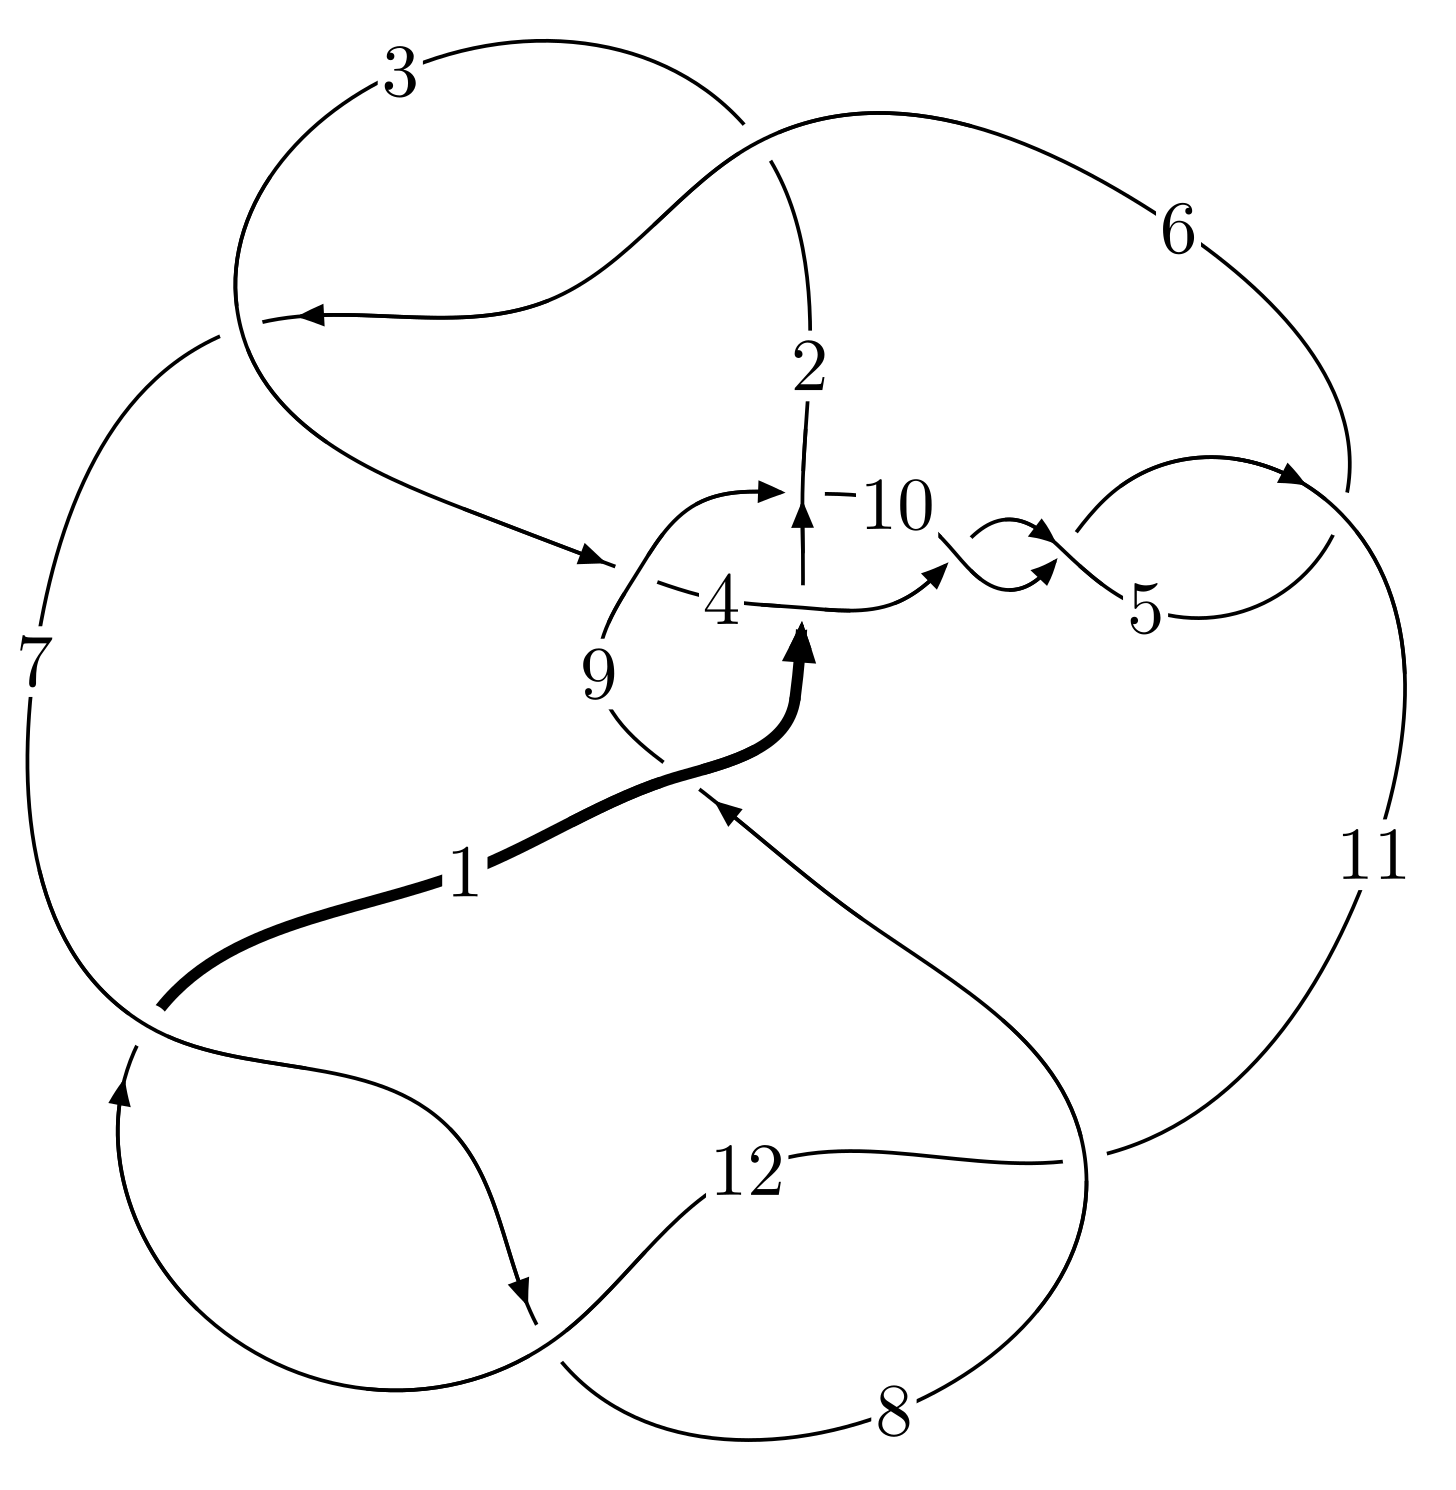
\includegraphics[width=112pt]{../../../GIT/diagram.site/Diagrams/png/1722_12a_0921.png}\\
\ \ \ A knot diagram\footnotemark}&
\allowdisplaybreaks
\textbf{Linearized knot diagam} \\
\cline{2-2}
 &
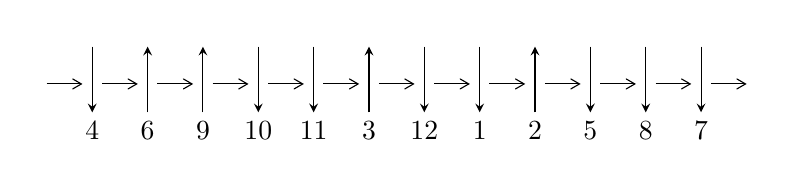
\begin{tikzpicture}[x=20pt, y=17pt]
	% nodes
	\node (C0) at (0, 0) {};
	\node (C1) at (1, 0) {};
	\node (C1U) at (1, +1) {};
	\node (C1D) at (1, -1) {4};

	\node (C2) at (2, 0) {};
	\node (C2U) at (2, +1) {};
	\node (C2D) at (2, -1) {6};

	\node (C3) at (3, 0) {};
	\node (C3U) at (3, +1) {};
	\node (C3D) at (3, -1) {9};

	\node (C4) at (4, 0) {};
	\node (C4U) at (4, +1) {};
	\node (C4D) at (4, -1) {10};

	\node (C5) at (5, 0) {};
	\node (C5U) at (5, +1) {};
	\node (C5D) at (5, -1) {11};

	\node (C6) at (6, 0) {};
	\node (C6U) at (6, +1) {};
	\node (C6D) at (6, -1) {3};

	\node (C7) at (7, 0) {};
	\node (C7U) at (7, +1) {};
	\node (C7D) at (7, -1) {12};

	\node (C8) at (8, 0) {};
	\node (C8U) at (8, +1) {};
	\node (C8D) at (8, -1) {1};

	\node (C9) at (9, 0) {};
	\node (C9U) at (9, +1) {};
	\node (C9D) at (9, -1) {2};

	\node (C10) at (10, 0) {};
	\node (C10U) at (10, +1) {};
	\node (C10D) at (10, -1) {5};

	\node (C11) at (11, 0) {};
	\node (C11U) at (11, +1) {};
	\node (C11D) at (11, -1) {8};

	\node (C12) at (12, 0) {};
	\node (C12U) at (12, +1) {};
	\node (C12D) at (12, -1) {7};
	\node (C13) at (13, 0) {};

	% arrows
	\draw[->,>={angle 60}]
	(C0) edge (C1) (C1) edge (C2) (C2) edge (C3) (C3) edge (C4) (C4) edge (C5) (C5) edge (C6) (C6) edge (C7) (C7) edge (C8) (C8) edge (C9) (C9) edge (C10) (C10) edge (C11) (C11) edge (C12) (C12) edge (C13) ;	\draw[->,>=stealth]
	(C1U) edge (C1D) (C2D) edge (C2U) (C3D) edge (C3U) (C4U) edge (C4D) (C5U) edge (C5D) (C6D) edge (C6U) (C7U) edge (C7D) (C8U) edge (C8D) (C9D) edge (C9U) (C10U) edge (C10D) (C11U) edge (C11D) (C12U) edge (C12D) ;
	\end{tikzpicture} \\
\hhline{~~} \\& 
\textbf{Solving Sequence} \\ \cline{2-2} 
 &
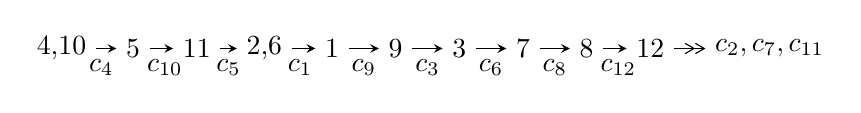
\begin{tikzpicture}[x=23pt, y=7pt]
	% node
	\node (A0) at (-1/8, 0) {4,10};
	\node (A1) at (1, 0) {5};
	\node (A2) at (2, 0) {11};
	\node (A3) at (49/16, 0) {2,6};
	\node (A4) at (33/8, 0) {1};
	\node (A5) at (41/8, 0) {9};
	\node (A6) at (49/8, 0) {3};
	\node (A7) at (57/8, 0) {7};
	\node (A8) at (65/8, 0) {8};
	\node (A9) at (73/8, 0) {12};
	\node (C1) at (1/2, -1) {$c_{4}$};
	\node (C2) at (3/2, -1) {$c_{10}$};
	\node (C3) at (5/2, -1) {$c_{5}$};
	\node (C4) at (29/8, -1) {$c_{1}$};
	\node (C5) at (37/8, -1) {$c_{9}$};
	\node (C6) at (45/8, -1) {$c_{3}$};
	\node (C7) at (53/8, -1) {$c_{6}$};
	\node (C8) at (61/8, -1) {$c_{8}$};
	\node (C9) at (69/8, -1) {$c_{12}$};
	\node (A10) at (11, 0) {$c_{2},c_{7},c_{11}$};

	% edge
	\draw[->,>=stealth]	
	(A0) edge (A1) (A1) edge (A2) (A2) edge (A3) (A3) edge (A4) (A4) edge (A5) (A5) edge (A6) (A6) edge (A7) (A7) edge (A8) (A8) edge (A9) ;
	\draw[->>,>={angle 60}]	
	(A9) edge (A10);
\end{tikzpicture} \\ 

\end{tabular} \\

\footnotetext{
The image of knot diagram is generated by the software ``\textbf{Draw programme}" developed by Andrew Bartholomew(\url{http://www.layer8.co.uk/maths/draw/index.htm\#Running-draw}), where we modified some parts for our purpose(\url{https://github.com/CATsTAILs/LinksPainter}).
}\phantom \\ \newline 
\centering \textbf{Ideals for irreducible components\footnotemark of $X_{\text{par}}$} 
 
\begin{align*}
I^u_{1}&=\langle 
-9.48478\times10^{151} u^{92}+2.29231\times10^{151} u^{91}+\cdots+4.90569\times10^{151} b-2.80006\times10^{152},\\
\phantom{I^u_{1}}&\phantom{= \langle  }2.01917\times10^{152} u^{92}-3.99607\times10^{151} u^{91}+\cdots+9.81138\times10^{151} a+9.96934\times10^{152},\;u^{93}+u^{92}+\cdots-18 u+4\rangle \\
I^u_{2}&=\langle 
u^{20}-9 u^{18}+\cdots-2 u^2+b,\;- u^{19}+10 u^{17}+\cdots+a+3,\;u^{21}-11 u^{19}+\cdots-6 u^2+1\rangle \\
I^u_{3}&=\langle 
- u^2+b,\;a-1,\;u^{15}-3 u^{13}+u^{10}+5 u^9-2 u^8- u^6-3 u^5+2 u^4- u^3+u^2-1\rangle \\
\\
\end{align*}
\raggedright * 3 irreducible components of $\dim_{\mathbb{C}}=0$, with total 129 representations.\\
\footnotetext{All coefficients of polynomials are rational numbers. But the coefficients are sometimes approximated in decimal forms when there is not enough margin.}
\newpage
\renewcommand{\arraystretch}{1}
\centering \section*{I. $I^u_{1}= \langle -9.48\times10^{151} u^{92}+2.29\times10^{151} u^{91}+\cdots+4.91\times10^{151} b-2.80\times10^{152},\;2.02\times10^{152} u^{92}-4.00\times10^{151} u^{91}+\cdots+9.81\times10^{151} a+9.97\times10^{152},\;u^{93}+u^{92}+\cdots-18 u+4 \rangle$}
\flushleft \textbf{(i) Arc colorings}\\
\begin{tabular}{m{7pt} m{180pt} m{7pt} m{180pt} }
\flushright $a_{4}=$&$\begin{pmatrix}1\\0\end{pmatrix}$ \\
\flushright $a_{10}=$&$\begin{pmatrix}0\\u\end{pmatrix}$ \\
\flushright $a_{5}=$&$\begin{pmatrix}1\\u^2\end{pmatrix}$ \\
\flushright $a_{11}=$&$\begin{pmatrix}- u\\- u^3+u\end{pmatrix}$ \\
\flushright $a_{2}=$&$\begin{pmatrix}-2.05799 u^{92}+0.407289 u^{91}+\cdots+12.6723 u-10.1610\\1.93342 u^{92}-0.467276 u^{91}+\cdots-30.7332 u+5.70778\end{pmatrix}$ \\
\flushright $a_{6}=$&$\begin{pmatrix}- u^2+1\\- u^4+2 u^2\end{pmatrix}$ \\
\flushright $a_{1}=$&$\begin{pmatrix}-0.124563 u^{92}-0.0599871 u^{91}+\cdots-18.0609 u-4.45321\\1.93342 u^{92}-0.467276 u^{91}+\cdots-30.7332 u+5.70778\end{pmatrix}$ \\
\flushright $a_{9}=$&$\begin{pmatrix}0.799139 u^{92}-0.728059 u^{91}+\cdots-46.3661 u+4.77657\\1.44094 u^{92}-0.629335 u^{91}+\cdots-29.6189 u+5.05852\end{pmatrix}$ \\
\flushright $a_{3}=$&$\begin{pmatrix}-1.94848 u^{92}+0.489593 u^{91}+\cdots+11.8488 u-10.0698\\1.92816 u^{92}-0.456854 u^{91}+\cdots-30.4428 u+5.56450\end{pmatrix}$ \\
\flushright $a_{7}=$&$\begin{pmatrix}1.25578 u^{92}-0.230053 u^{91}+\cdots-14.2454 u-1.89595\\-1.36128 u^{92}+0.166064 u^{91}+\cdots+17.7972 u-4.51459\end{pmatrix}$ \\
\flushright $a_{8}=$&$\begin{pmatrix}-1.51946 u^{92}+0.0968024 u^{91}+\cdots+24.1105 u-2.93910\\-2.91059 u^{92}+0.633840 u^{91}+\cdots+41.0680 u-8.34160\end{pmatrix}$ \\
\flushright $a_{12}=$&$\begin{pmatrix}0.632413 u^{92}-0.385835 u^{91}+\cdots-27.7370 u+0.504505\\-0.480647 u^{92}+0.112108 u^{91}+\cdots-0.601988 u+0.0953933\end{pmatrix}$\\&\end{tabular}
\flushleft \textbf{(ii) Obstruction class $= -1$}\\~\\
\flushleft \textbf{(iii) Cusp Shapes $= -4.79061 u^{92}+1.91185 u^{91}+\cdots+111.874 u-20.5189$}\\~\\
\newpage\renewcommand{\arraystretch}{1}
\flushleft \textbf{(iv) u-Polynomials at the component}\newline \\
\begin{tabular}{m{50pt}|m{274pt}}
Crossings & \hspace{64pt}u-Polynomials at each crossing \\
\hline $$\begin{aligned}c_{1}\end{aligned}$$&$\begin{aligned}
&u^{93}-7 u^{92}+\cdots+87046 u-14548
\end{aligned}$\\
\hline $$\begin{aligned}c_{2},c_{6}\end{aligned}$$&$\begin{aligned}
&u^{93}-4 u^{92}+\cdots+818 u+292
\end{aligned}$\\
\hline $$\begin{aligned}c_{3}\end{aligned}$$&$\begin{aligned}
&u^{93}- u^{92}+\cdots+82 u-4
\end{aligned}$\\
\hline $$\begin{aligned}c_{4},c_{5},c_{10}\end{aligned}$$&$\begin{aligned}
&u^{93}+u^{92}+\cdots-18 u+4
\end{aligned}$\\
\hline $$\begin{aligned}c_{7},c_{11},c_{12}\end{aligned}$$&$\begin{aligned}
&u^{93}-5 u^{92}+\cdots-62 u+4
\end{aligned}$\\
\hline $$\begin{aligned}c_{8}\end{aligned}$$&$\begin{aligned}
&u^{93}+5 u^{92}+\cdots-263654 u+40564
\end{aligned}$\\
\hline $$\begin{aligned}c_{9}\end{aligned}$$&$\begin{aligned}
&u^{93}+3 u^{92}+\cdots-3506 u-1364
\end{aligned}$\\
\hline
\end{tabular}\\~\\
\newpage\renewcommand{\arraystretch}{1}
\flushleft \textbf{(v) Riley Polynomials at the component}\newline \\
\begin{tabular}{m{50pt}|m{274pt}}
Crossings & \hspace{64pt}Riley Polynomials at each crossing \\
\hline $$\begin{aligned}c_{1}\end{aligned}$$&$\begin{aligned}
&y^{93}-19 y^{92}+\cdots+9425154940 y-211644304
\end{aligned}$\\
\hline $$\begin{aligned}c_{2},c_{6}\end{aligned}$$&$\begin{aligned}
&y^{93}-48 y^{92}+\cdots+1643820 y-85264
\end{aligned}$\\
\hline $$\begin{aligned}c_{3}\end{aligned}$$&$\begin{aligned}
&y^{93}-9 y^{92}+\cdots+3164 y-16
\end{aligned}$\\
\hline $$\begin{aligned}c_{4},c_{5},c_{10}\end{aligned}$$&$\begin{aligned}
&y^{93}-101 y^{92}+\cdots-468 y-16
\end{aligned}$\\
\hline $$\begin{aligned}c_{7},c_{11},c_{12}\end{aligned}$$&$\begin{aligned}
&y^{93}+81 y^{92}+\cdots+588 y-16
\end{aligned}$\\
\hline $$\begin{aligned}c_{8}\end{aligned}$$&$\begin{aligned}
&y^{93}-27 y^{92}+\cdots+67097196492 y-1645438096
\end{aligned}$\\
\hline $$\begin{aligned}c_{9}\end{aligned}$$&$\begin{aligned}
&y^{93}+21 y^{92}+\cdots-67270084 y-1860496
\end{aligned}$\\
\hline
\end{tabular}\\~\\
\newpage\flushleft \textbf{(vi) Complex Volumes and Cusp Shapes}
$$\begin{array}{c|c|c}  
\text{Solutions to }I^u_{1}& \I (\text{vol} + \sqrt{-1}CS) & \text{Cusp shape}\\
 \hline 
\begin{aligned}
u &= -0.508441 + 0.865954 I \\
a &= -0.325096 + 1.247810 I \\
b &= \phantom{-}1.041020 - 0.783812 I\end{aligned}
 & \phantom{-}0.20096 + 8.92280 I & \phantom{-0.000000 } 0 \\ \hline\begin{aligned}
u &= -0.508441 - 0.865954 I \\
a &= -0.325096 - 1.247810 I \\
b &= \phantom{-}1.041020 + 0.783812 I\end{aligned}
 & \phantom{-}0.20096 - 8.92280 I & \phantom{-0.000000 } 0 \\ \hline\begin{aligned}
u &= \phantom{-}0.469257 + 0.915218 I \\
a &= -0.423152 - 1.219970 I \\
b &= \phantom{-}1.082360 + 0.876290 I\end{aligned}
 & \phantom{-}5.41996 - 12.97790 I & \phantom{-0.000000 } 0 \\ \hline\begin{aligned}
u &= \phantom{-}0.469257 - 0.915218 I \\
a &= -0.423152 + 1.219970 I \\
b &= \phantom{-}1.082360 - 0.876290 I\end{aligned}
 & \phantom{-}5.41996 + 12.97790 I & \phantom{-0.000000 } 0 \\ \hline\begin{aligned}
u &= -0.927529 + 0.448886 I \\
a &= -1.058270 + 0.051455 I \\
b &= \phantom{-}0.397945 + 0.501367 I\end{aligned}
 & \phantom{-}8.09310 + 0.14930 I & \phantom{-0.000000 } 0 \\ \hline\begin{aligned}
u &= -0.927529 - 0.448886 I \\
a &= -1.058270 - 0.051455 I \\
b &= \phantom{-}0.397945 - 0.501367 I\end{aligned}
 & \phantom{-}8.09310 - 0.14930 I & \phantom{-0.000000 } 0 \\ \hline\begin{aligned}
u &= \phantom{-}0.530707 + 0.896493 I \\
a &= -0.490200 + 0.098599 I \\
b &= \phantom{-}0.718569 - 0.370152 I\end{aligned}
 & \phantom{-}2.47227 - 0.63691 I & \phantom{-0.000000 } 0 \\ \hline\begin{aligned}
u &= \phantom{-}0.530707 - 0.896493 I \\
a &= -0.490200 - 0.098599 I \\
b &= \phantom{-}0.718569 + 0.370152 I\end{aligned}
 & \phantom{-}2.47227 + 0.63691 I & \phantom{-0.000000 } 0 \\ \hline\begin{aligned}
u &= \phantom{-}0.534102 + 0.752303 I \\
a &= -0.142930 - 1.371140 I \\
b &= \phantom{-}0.918907 + 0.670898 I\end{aligned}
 & \phantom{-}2.25254 - 4.57716 I & \phantom{-0.000000 } 0 \\ \hline\begin{aligned}
u &= \phantom{-}0.534102 - 0.752303 I \\
a &= -0.142930 + 1.371140 I \\
b &= \phantom{-}0.918907 - 0.670898 I\end{aligned}
 & \phantom{-}2.25254 + 4.57716 I & \phantom{-0.000000 } 0\\
 \hline 
 \end{array}$$\newpage$$\begin{array}{c|c|c}  
\text{Solutions to }I^u_{1}& \I (\text{vol} + \sqrt{-1}CS) & \text{Cusp shape}\\
 \hline 
\begin{aligned}
u &= -0.735519 + 0.867109 I \\
a &= -0.628196 + 0.018969 I \\
b &= \phantom{-}0.763287 + 0.500011 I\end{aligned}
 & -0.33868 - 3.16041 I & \phantom{-0.000000 } 0 \\ \hline\begin{aligned}
u &= -0.735519 - 0.867109 I \\
a &= -0.628196 - 0.018969 I \\
b &= \phantom{-}0.763287 - 0.500011 I\end{aligned}
 & -0.33868 + 3.16041 I & \phantom{-0.000000 } 0 \\ \hline\begin{aligned}
u &= -0.556116 + 0.577176 I \\
a &= \phantom{-}0.178244 - 1.271710 I \\
b &= -1.08666 + 0.99348 I\end{aligned}
 & \phantom{-}2.06421 + 7.25817 I & \phantom{-0.000000 } 0 \\ \hline\begin{aligned}
u &= -0.556116 - 0.577176 I \\
a &= \phantom{-}0.178244 + 1.271710 I \\
b &= -1.08666 - 0.99348 I\end{aligned}
 & \phantom{-}2.06421 - 7.25817 I & \phantom{-0.000000 } 0 \\ \hline\begin{aligned}
u &= \phantom{-}0.837532 + 0.861025 I \\
a &= -0.678478 - 0.091597 I \\
b &= \phantom{-}0.777681 - 0.589874 I\end{aligned}
 & \phantom{-}4.46674 + 7.02318 I & \phantom{-0.000000 } 0 \\ \hline\begin{aligned}
u &= \phantom{-}0.837532 - 0.861025 I \\
a &= -0.678478 + 0.091597 I \\
b &= \phantom{-}0.777681 + 0.589874 I\end{aligned}
 & \phantom{-}4.46674 - 7.02318 I & \phantom{-0.000000 } 0 \\ \hline\begin{aligned}
u &= \phantom{-}0.625041 + 0.460913 I \\
a &= \phantom{-}0.66228 - 1.43861 I \\
b &= \phantom{-}0.745720 + 0.381896 I\end{aligned}
 & \phantom{-}1.99795 - 3.83741 I & \phantom{-0.000000 } 0 \\ \hline\begin{aligned}
u &= \phantom{-}0.625041 - 0.460913 I \\
a &= \phantom{-}0.66228 + 1.43861 I \\
b &= \phantom{-}0.745720 - 0.381896 I\end{aligned}
 & \phantom{-}1.99795 + 3.83741 I & \phantom{-0.000000 } 0 \\ \hline\begin{aligned}
u &= -0.301204 + 0.688922 I \\
a &= -0.56454 + 1.82402 I \\
b &= \phantom{-}0.624251 - 0.868525 I\end{aligned}
 & \phantom{-}9.88119 + 3.92848 I & \phantom{-0.000000 } 0 \\ \hline\begin{aligned}
u &= -0.301204 - 0.688922 I \\
a &= -0.56454 - 1.82402 I \\
b &= \phantom{-}0.624251 + 0.868525 I\end{aligned}
 & \phantom{-}9.88119 - 3.92848 I & \phantom{-0.000000 } 0\\
 \hline 
 \end{array}$$\newpage$$\begin{array}{c|c|c}  
\text{Solutions to }I^u_{1}& \I (\text{vol} + \sqrt{-1}CS) & \text{Cusp shape}\\
 \hline 
\begin{aligned}
u &= -0.723386\phantom{ +0.000000I} \\
a &= \phantom{-}1.60032\phantom{ +0.000000I} \\
b &= \phantom{-}0.704568\phantom{ +0.000000I}\end{aligned}
 & -0.943143\phantom{ +0.000000I} & -10.4180\phantom{ +0.000000I} \\ \hline\begin{aligned}
u &= -1.281680 + 0.000599 I \\
a &= -0.204360 + 1.175340 I \\
b &= -0.788781 - 1.123720 I\end{aligned}
 & \phantom{-}1.54277 - 5.13635 I & \phantom{-0.000000 } 0 \\ \hline\begin{aligned}
u &= -1.281680 - 0.000599 I \\
a &= -0.204360 - 1.175340 I \\
b &= -0.788781 + 1.123720 I\end{aligned}
 & \phantom{-}1.54277 + 5.13635 I & \phantom{-0.000000 } 0 \\ \hline\begin{aligned}
u &= \phantom{-}0.538824 + 0.470683 I \\
a &= \phantom{-}0.160205 + 1.374300 I \\
b &= -1.080240 - 0.790479 I\end{aligned}
 & -2.76079 - 3.81720 I & -9.13434 + 6.95796 I \\ \hline\begin{aligned}
u &= \phantom{-}0.538824 - 0.470683 I \\
a &= \phantom{-}0.160205 - 1.374300 I \\
b &= -1.080240 + 0.790479 I\end{aligned}
 & -2.76079 + 3.81720 I & -9.13434 - 6.95796 I \\ \hline\begin{aligned}
u &= \phantom{-}0.260333 + 0.634297 I \\
a &= \phantom{-}0.292242 + 1.114540 I \\
b &= -0.257972 - 1.062420 I\end{aligned}
 & \phantom{-}4.35474 - 0.70676 I & \phantom{-}1.78969 + 4.36362 I \\ \hline\begin{aligned}
u &= \phantom{-}0.260333 - 0.634297 I \\
a &= \phantom{-}0.292242 - 1.114540 I \\
b &= -0.257972 + 1.062420 I\end{aligned}
 & \phantom{-}4.35474 + 0.70676 I & \phantom{-}1.78969 - 4.36362 I \\ \hline\begin{aligned}
u &= -1.316730 + 0.162695 I \\
a &= -0.170965 - 0.295963 I \\
b &= \phantom{-}0.30737 + 2.10149 I\end{aligned}
 & \phantom{-}2.22557 + 8.18081 I & \phantom{-0.000000 } 0 \\ \hline\begin{aligned}
u &= -1.316730 - 0.162695 I \\
a &= -0.170965 + 0.295963 I \\
b &= \phantom{-}0.30737 - 2.10149 I\end{aligned}
 & \phantom{-}2.22557 - 8.18081 I & \phantom{-0.000000 } 0 \\ \hline\begin{aligned}
u &= \phantom{-}1.326910 + 0.070082 I \\
a &= -0.001160 + 0.218282 I \\
b &= \phantom{-}1.26981 - 1.26624 I\end{aligned}
 & \phantom{-}3.28953 + 0.55896 I & \phantom{-0.000000 } 0\\
 \hline 
 \end{array}$$\newpage$$\begin{array}{c|c|c}  
\text{Solutions to }I^u_{1}& \I (\text{vol} + \sqrt{-1}CS) & \text{Cusp shape}\\
 \hline 
\begin{aligned}
u &= \phantom{-}1.326910 - 0.070082 I \\
a &= -0.001160 - 0.218282 I \\
b &= \phantom{-}1.26981 + 1.26624 I\end{aligned}
 & \phantom{-}3.28953 - 0.55896 I & \phantom{-0.000000 } 0 \\ \hline\begin{aligned}
u &= -1.281140 + 0.367616 I \\
a &= -0.069228 - 0.910131 I \\
b &= -1.28880 + 0.64130 I\end{aligned}
 & -0.63612 + 2.02419 I & \phantom{-0.000000 } 0 \\ \hline\begin{aligned}
u &= -1.281140 - 0.367616 I \\
a &= -0.069228 + 0.910131 I \\
b &= -1.28880 - 0.64130 I\end{aligned}
 & -0.63612 - 2.02419 I & \phantom{-0.000000 } 0 \\ \hline\begin{aligned}
u &= \phantom{-}1.353450 + 0.161844 I \\
a &= -0.132542 + 0.363700 I \\
b &= \phantom{-}0.17474 - 1.64951 I\end{aligned}
 & -3.22563 - 5.08058 I & \phantom{-0.000000 } 0 \\ \hline\begin{aligned}
u &= \phantom{-}1.353450 - 0.161844 I \\
a &= -0.132542 - 0.363700 I \\
b &= \phantom{-}0.17474 + 1.64951 I\end{aligned}
 & -3.22563 + 5.08058 I & \phantom{-0.000000 } 0 \\ \hline\begin{aligned}
u &= \phantom{-}0.407933 + 0.464047 I \\
a &= -0.866007 + 0.691674 I \\
b &= \phantom{-}0.688589 - 0.455821 I\end{aligned}
 & \phantom{-}2.66989 + 0.13790 I & \phantom{-}2.92063 - 0.32720 I \\ \hline\begin{aligned}
u &= \phantom{-}0.407933 - 0.464047 I \\
a &= -0.866007 - 0.691674 I \\
b &= \phantom{-}0.688589 + 0.455821 I\end{aligned}
 & \phantom{-}2.66989 - 0.13790 I & \phantom{-}2.92063 + 0.32720 I \\ \hline\begin{aligned}
u &= -1.381120 + 0.098816 I \\
a &= \phantom{-}0.006521 - 0.340348 I \\
b &= \phantom{-}0.636543 + 1.106670 I\end{aligned}
 & -2.64960 + 1.68388 I & \phantom{-0.000000 } 0 \\ \hline\begin{aligned}
u &= -1.381120 - 0.098816 I \\
a &= \phantom{-}0.006521 + 0.340348 I \\
b &= \phantom{-}0.636543 - 1.106670 I\end{aligned}
 & -2.64960 - 1.68388 I & \phantom{-0.000000 } 0 \\ \hline\begin{aligned}
u &= \phantom{-}1.360210 + 0.260057 I \\
a &= -0.162811 + 0.802512 I \\
b &= -1.021440 - 0.796484 I\end{aligned}
 & -4.89754 - 3.66913 I & \phantom{-0.000000 } 0\\
 \hline 
 \end{array}$$\newpage$$\begin{array}{c|c|c}  
\text{Solutions to }I^u_{1}& \I (\text{vol} + \sqrt{-1}CS) & \text{Cusp shape}\\
 \hline 
\begin{aligned}
u &= \phantom{-}1.360210 - 0.260057 I \\
a &= -0.162811 - 0.802512 I \\
b &= -1.021440 + 0.796484 I\end{aligned}
 & -4.89754 + 3.66913 I & \phantom{-0.000000 } 0 \\ \hline\begin{aligned}
u &= \phantom{-}1.389140 + 0.012717 I \\
a &= -0.554931 + 1.201120 I \\
b &= -0.847473 - 0.644385 I\end{aligned}
 & -5.08356 - 2.17532 I & \phantom{-0.000000 } 0 \\ \hline\begin{aligned}
u &= \phantom{-}1.389140 - 0.012717 I \\
a &= -0.554931 - 1.201120 I \\
b &= -0.847473 + 0.644385 I\end{aligned}
 & -5.08356 + 2.17532 I & \phantom{-0.000000 } 0 \\ \hline\begin{aligned}
u &= \phantom{-}1.406690 + 0.094426 I \\
a &= -1.29452 - 1.03273 I \\
b &= -0.598145 - 0.021332 I\end{aligned}
 & -0.18126 - 7.44744 I & \phantom{-0.000000 } 0 \\ \hline\begin{aligned}
u &= \phantom{-}1.406690 - 0.094426 I \\
a &= -1.29452 + 1.03273 I \\
b &= -0.598145 + 0.021332 I\end{aligned}
 & -0.18126 + 7.44744 I & \phantom{-0.000000 } 0 \\ \hline\begin{aligned}
u &= -1.39601 + 0.23784 I \\
a &= -0.329690 - 0.575972 I \\
b &= -0.98291 + 1.39370 I\end{aligned}
 & -0.90850 + 3.86973 I & \phantom{-0.000000 } 0 \\ \hline\begin{aligned}
u &= -1.39601 - 0.23784 I \\
a &= -0.329690 + 0.575972 I \\
b &= -0.98291 - 1.39370 I\end{aligned}
 & -0.90850 - 3.86973 I & \phantom{-0.000000 } 0 \\ \hline\begin{aligned}
u &= -1.41760 + 0.04823 I \\
a &= -0.99595 + 1.26314 I \\
b &= -0.693903 - 0.244095 I\end{aligned}
 & -6.04675 + 2.86647 I & \phantom{-0.000000 } 0 \\ \hline\begin{aligned}
u &= -1.41760 - 0.04823 I \\
a &= -0.99595 - 1.26314 I \\
b &= -0.693903 + 0.244095 I\end{aligned}
 & -6.04675 - 2.86647 I & \phantom{-0.000000 } 0 \\ \hline\begin{aligned}
u &= -0.135731 + 0.564632 I \\
a &= -0.038430 - 1.246730 I \\
b &= \phantom{-}0.596702 + 1.029200 I\end{aligned}
 & \phantom{-}1.44493 + 2.51937 I & \phantom{-}0.01028 - 7.23544 I\\
 \hline 
 \end{array}$$\newpage$$\begin{array}{c|c|c}  
\text{Solutions to }I^u_{1}& \I (\text{vol} + \sqrt{-1}CS) & \text{Cusp shape}\\
 \hline 
\begin{aligned}
u &= -0.135731 - 0.564632 I \\
a &= -0.038430 + 1.246730 I \\
b &= \phantom{-}0.596702 - 1.029200 I\end{aligned}
 & \phantom{-}1.44493 - 2.51937 I & \phantom{-}0.01028 + 7.23544 I \\ \hline\begin{aligned}
u &= \phantom{-}0.047256 + 0.569881 I \\
a &= \phantom{-}0.11875 + 1.41024 I \\
b &= \phantom{-}0.79856 - 1.28376 I\end{aligned}
 & \phantom{-}6.45729 - 5.60603 I & \phantom{-}5.38089 + 6.61393 I \\ \hline\begin{aligned}
u &= \phantom{-}0.047256 - 0.569881 I \\
a &= \phantom{-}0.11875 - 1.41024 I \\
b &= \phantom{-}0.79856 + 1.28376 I\end{aligned}
 & \phantom{-}6.45729 + 5.60603 I & \phantom{-}5.38089 - 6.61393 I \\ \hline\begin{aligned}
u &= \phantom{-}1.43982 + 0.23261 I \\
a &= \phantom{-}0.553535 - 1.141840 I \\
b &= \phantom{-}0.815368 + 1.022160 I\end{aligned}
 & \phantom{-}4.25414 - 7.21931 I & \phantom{-0.000000 } 0 \\ \hline\begin{aligned}
u &= \phantom{-}1.43982 - 0.23261 I \\
a &= \phantom{-}0.553535 + 1.141840 I \\
b &= \phantom{-}0.815368 - 1.022160 I\end{aligned}
 & \phantom{-}4.25414 + 7.21931 I & \phantom{-0.000000 } 0 \\ \hline\begin{aligned}
u &= -0.467586 + 0.257946 I \\
a &= \phantom{-}0.02407 - 1.81471 I \\
b &= -1.094560 + 0.380639 I\end{aligned}
 & -0.223024 + 0.638682 I & -7.26593 - 1.08990 I \\ \hline\begin{aligned}
u &= -0.467586 - 0.257946 I \\
a &= \phantom{-}0.02407 + 1.81471 I \\
b &= -1.094560 - 0.380639 I\end{aligned}
 & -0.223024 - 0.638682 I & -7.26593 + 1.08990 I \\ \hline\begin{aligned}
u &= \phantom{-}1.48280 + 0.12522 I \\
a &= -0.584483 + 0.824508 I \\
b &= -1.39781 - 0.71566 I\end{aligned}
 & -6.64297 - 2.24828 I & \phantom{-0.000000 } 0 \\ \hline\begin{aligned}
u &= \phantom{-}1.48280 - 0.12522 I \\
a &= -0.584483 - 0.824508 I \\
b &= -1.39781 + 0.71566 I\end{aligned}
 & -6.64297 + 2.24828 I & \phantom{-0.000000 } 0 \\ \hline\begin{aligned}
u &= -1.49936 + 0.17405 I \\
a &= -0.571538 - 0.743869 I \\
b &= -1.53989 + 0.86367 I\end{aligned}
 & -9.39431 + 6.26075 I & \phantom{-0.000000 } 0\\
 \hline 
 \end{array}$$\newpage$$\begin{array}{c|c|c}  
\text{Solutions to }I^u_{1}& \I (\text{vol} + \sqrt{-1}CS) & \text{Cusp shape}\\
 \hline 
\begin{aligned}
u &= -1.49936 - 0.17405 I \\
a &= -0.571538 + 0.743869 I \\
b &= -1.53989 - 0.86367 I\end{aligned}
 & -9.39431 - 6.26075 I & \phantom{-0.000000 } 0 \\ \hline\begin{aligned}
u &= \phantom{-}1.50553 + 0.20623 I \\
a &= -0.567957 + 0.697438 I \\
b &= -1.62262 - 0.98031 I\end{aligned}
 & -4.61612 - 10.16490 I & \phantom{-0.000000 } 0 \\ \hline\begin{aligned}
u &= \phantom{-}1.50553 - 0.20623 I \\
a &= -0.567957 - 0.697438 I \\
b &= -1.62262 + 0.98031 I\end{aligned}
 & -4.61612 + 10.16490 I & \phantom{-0.000000 } 0 \\ \hline\begin{aligned}
u &= \phantom{-}1.48132 + 0.41379 I \\
a &= \phantom{-}0.044885 + 0.816597 I \\
b &= -1.072630 - 0.146328 I\end{aligned}
 & -2.25116 - 8.01558 I & \phantom{-0.000000 } 0 \\ \hline\begin{aligned}
u &= \phantom{-}1.48132 - 0.41379 I \\
a &= \phantom{-}0.044885 - 0.816597 I \\
b &= -1.072630 + 0.146328 I\end{aligned}
 & -2.25116 + 8.01558 I & \phantom{-0.000000 } 0 \\ \hline\begin{aligned}
u &= -1.49735 + 0.35692 I \\
a &= \phantom{-}0.039185 - 0.774715 I \\
b &= -0.871253 + 0.182705 I\end{aligned}
 & -6.70226 + 4.67739 I & \phantom{-0.000000 } 0 \\ \hline\begin{aligned}
u &= -1.49735 - 0.35692 I \\
a &= \phantom{-}0.039185 + 0.774715 I \\
b &= -0.871253 - 0.182705 I\end{aligned}
 & -6.70226 - 4.67739 I & \phantom{-0.000000 } 0 \\ \hline\begin{aligned}
u &= -1.53475 + 0.12089 I \\
a &= \phantom{-}1.024310 + 0.928571 I \\
b &= \phantom{-}0.722740 - 0.376986 I\end{aligned}
 & -5.12025 + 5.82093 I & \phantom{-0.000000 } 0 \\ \hline\begin{aligned}
u &= -1.53475 - 0.12089 I \\
a &= \phantom{-}1.024310 - 0.928571 I \\
b &= \phantom{-}0.722740 + 0.376986 I\end{aligned}
 & -5.12025 - 5.82093 I & \phantom{-0.000000 } 0 \\ \hline\begin{aligned}
u &= -1.52693 + 0.26895 I \\
a &= \phantom{-}0.586700 + 0.990447 I \\
b &= \phantom{-}1.170260 - 0.787437 I\end{aligned}
 & -4.44470 + 8.33731 I & \phantom{-0.000000 } 0\\
 \hline 
 \end{array}$$\newpage$$\begin{array}{c|c|c}  
\text{Solutions to }I^u_{1}& \I (\text{vol} + \sqrt{-1}CS) & \text{Cusp shape}\\
 \hline 
\begin{aligned}
u &= -1.52693 - 0.26895 I \\
a &= \phantom{-}0.586700 - 0.990447 I \\
b &= \phantom{-}1.170260 + 0.787437 I\end{aligned}
 & -4.44470 - 8.33731 I & \phantom{-0.000000 } 0 \\ \hline\begin{aligned}
u &= -0.235303 + 0.381265 I \\
a &= \phantom{-}0.96159 - 1.43797 I \\
b &= -0.610180 + 0.360523 I\end{aligned}
 & -0.375586 + 1.110620 I & -5.85320 - 5.23683 I \\ \hline\begin{aligned}
u &= -0.235303 - 0.381265 I \\
a &= \phantom{-}0.96159 + 1.43797 I \\
b &= -0.610180 - 0.360523 I\end{aligned}
 & -0.375586 - 1.110620 I & -5.85320 + 5.23683 I \\ \hline\begin{aligned}
u &= -1.52414 + 0.33387 I \\
a &= \phantom{-}0.521304 + 0.976377 I \\
b &= \phantom{-}1.39892 - 0.94174 I\end{aligned}
 & -1.0116 + 17.5021 I & \phantom{-0.000000 } 0 \\ \hline\begin{aligned}
u &= -1.52414 - 0.33387 I \\
a &= \phantom{-}0.521304 - 0.976377 I \\
b &= \phantom{-}1.39892 + 0.94174 I\end{aligned}
 & -1.0116 - 17.5021 I & \phantom{-0.000000 } 0 \\ \hline\begin{aligned}
u &= \phantom{-}1.56065\phantom{ +0.000000I} \\
a &= \phantom{-}1.42405\phantom{ +0.000000I} \\
b &= \phantom{-}0.642348\phantom{ +0.000000I}\end{aligned}
 & -8.44045\phantom{ +0.000000I} & \phantom{-0.000000 } 0 \\ \hline\begin{aligned}
u &= \phantom{-}1.53200 + 0.30838 I \\
a &= \phantom{-}0.544303 - 0.975626 I \\
b &= \phantom{-}1.32328 + 0.85818 I\end{aligned}
 & -6.4092 - 13.1952 I & \phantom{-0.000000 } 0 \\ \hline\begin{aligned}
u &= \phantom{-}1.53200 - 0.30838 I \\
a &= \phantom{-}0.544303 + 0.975626 I \\
b &= \phantom{-}1.32328 - 0.85818 I\end{aligned}
 & -6.4092 + 13.1952 I & \phantom{-0.000000 } 0 \\ \hline\begin{aligned}
u &= \phantom{-}1.54225 + 0.29438 I \\
a &= \phantom{-}0.069262 + 0.717819 I \\
b &= -0.570637 - 0.119504 I\end{aligned}
 & -3.25509 - 1.51532 I & \phantom{-0.000000 } 0 \\ \hline\begin{aligned}
u &= \phantom{-}1.54225 - 0.29438 I \\
a &= \phantom{-}0.069262 - 0.717819 I \\
b &= -0.570637 + 0.119504 I\end{aligned}
 & -3.25509 + 1.51532 I & \phantom{-0.000000 } 0\\
 \hline 
 \end{array}$$\newpage$$\begin{array}{c|c|c}  
\text{Solutions to }I^u_{1}& \I (\text{vol} + \sqrt{-1}CS) & \text{Cusp shape}\\
 \hline 
\begin{aligned}
u &= -1.60036 + 0.03902 I \\
a &= \phantom{-}0.339371 + 0.487975 I \\
b &= \phantom{-}0.710583 - 0.058904 I\end{aligned}
 & -4.93556 - 4.01294 I & \phantom{-0.000000 } 0 \\ \hline\begin{aligned}
u &= -1.60036 - 0.03902 I \\
a &= \phantom{-}0.339371 - 0.487975 I \\
b &= \phantom{-}0.710583 + 0.058904 I\end{aligned}
 & -4.93556 + 4.01294 I & \phantom{-0.000000 } 0 \\ \hline\begin{aligned}
u &= \phantom{-}1.60243 + 0.10816 I \\
a &= \phantom{-}0.405139 - 0.408093 I \\
b &= \phantom{-}0.827639 + 0.088426 I\end{aligned}
 & -8.97902 - 0.30493 I & \phantom{-0.000000 } 0 \\ \hline\begin{aligned}
u &= \phantom{-}1.60243 - 0.10816 I \\
a &= \phantom{-}0.405139 + 0.408093 I \\
b &= \phantom{-}0.827639 - 0.088426 I\end{aligned}
 & -8.97902 + 0.30493 I & \phantom{-0.000000 } 0 \\ \hline\begin{aligned}
u &= -1.60735 + 0.20212 I \\
a &= \phantom{-}0.386947 + 0.314917 I \\
b &= \phantom{-}0.890916 - 0.105990 I\end{aligned}
 & -5.13275 + 4.82360 I & \phantom{-0.000000 } 0 \\ \hline\begin{aligned}
u &= -1.60735 - 0.20212 I \\
a &= \phantom{-}0.386947 - 0.314917 I \\
b &= \phantom{-}0.890916 + 0.105990 I\end{aligned}
 & -5.13275 - 4.82360 I & \phantom{-0.000000 } 0 \\ \hline\begin{aligned}
u &= \phantom{-}0.346577\phantom{ +0.000000I} \\
a &= -2.36075\phantom{ +0.000000I} \\
b &= \phantom{-}0.943840\phantom{ +0.000000I}\end{aligned}
 & \phantom{-}2.83068\phantom{ +0.000000I} & \phantom{-}10.4240\phantom{ +0.000000I} \\ \hline\begin{aligned}
u &= -0.152629 + 0.293549 I \\
a &= -4.52463 - 0.47527 I \\
b &= -0.490294 + 0.609024 I\end{aligned}
 & \phantom{-}4.95962 + 6.04460 I & \phantom{-}1.17092 - 11.50660 I \\ \hline\begin{aligned}
u &= -0.152629 - 0.293549 I \\
a &= -4.52463 + 0.47527 I \\
b &= -0.490294 - 0.609024 I\end{aligned}
 & \phantom{-}4.95962 - 6.04460 I & \phantom{-}1.17092 + 11.50660 I \\ \hline\begin{aligned}
u &= -0.008205 + 0.246331 I \\
a &= -0.08505 - 3.19265 I \\
b &= \phantom{-}1.45669 + 0.61935 I\end{aligned}
 & \phantom{-}7.62756 - 1.79977 I & \phantom{-}9.81021 + 0.38909 I\\
 \hline 
 \end{array}$$\newpage$$\begin{array}{c|c|c}  
\text{Solutions to }I^u_{1}& \I (\text{vol} + \sqrt{-1}CS) & \text{Cusp shape}\\
 \hline 
\begin{aligned}
u &= -0.008205 - 0.246331 I \\
a &= -0.08505 + 3.19265 I \\
b &= \phantom{-}1.45669 - 0.61935 I\end{aligned}
 & \phantom{-}7.62756 + 1.79977 I & \phantom{-}9.81021 - 0.38909 I \\ \hline\begin{aligned}
u &= \phantom{-}0.127305 + 0.126214 I \\
a &= -7.28555 - 3.50390 I \\
b &= -0.587613 - 0.256457 I\end{aligned}
 & -0.85046 - 2.18730 I & -11.9288 + 11.8413 I \\ \hline\begin{aligned}
u &= \phantom{-}0.127305 - 0.126214 I \\
a &= -7.28555 + 3.50390 I \\
b &= -0.587613 + 0.256457 I\end{aligned}
 & -0.85046 + 2.18730 I & -11.9288 - 11.8413 I\\
 \hline 
 \end{array}$$\newpage\newpage\renewcommand{\arraystretch}{1}
\centering \section*{II. $I^u_{2}= \langle u^{20}-9 u^{18}+\cdots-2 u^2+b,\;- u^{19}+10 u^{17}+\cdots+a+3,\;u^{21}-11 u^{19}+\cdots-6 u^2+1 \rangle$}
\flushleft \textbf{(i) Arc colorings}\\
\begin{tabular}{m{7pt} m{180pt} m{7pt} m{180pt} }
\flushright $a_{4}=$&$\begin{pmatrix}1\\0\end{pmatrix}$ \\
\flushright $a_{10}=$&$\begin{pmatrix}0\\u\end{pmatrix}$ \\
\flushright $a_{5}=$&$\begin{pmatrix}1\\u^2\end{pmatrix}$ \\
\flushright $a_{11}=$&$\begin{pmatrix}- u\\- u^3+u\end{pmatrix}$ \\
\flushright $a_{2}=$&$\begin{pmatrix}u^{19}-10 u^{17}+\cdots+9 u^2-3\\- u^{20}+9 u^{18}+\cdots- u^3+2 u^2\end{pmatrix}$ \\
\flushright $a_{6}=$&$\begin{pmatrix}- u^2+1\\- u^4+2 u^2\end{pmatrix}$ \\
\flushright $a_{1}=$&$\begin{pmatrix}- u^{20}+u^{19}+\cdots+11 u^2-3\\- u^{20}+9 u^{18}+\cdots- u^3+2 u^2\end{pmatrix}$ \\
\flushright $a_{9}=$&$\begin{pmatrix}-2 u^{18}+18 u^{16}+\cdots-2 u^2-3 u\\u^{19}-10 u^{17}+\cdots+2 u-1\end{pmatrix}$ \\
\flushright $a_{3}=$&$\begin{pmatrix}u^{19}-10 u^{17}+\cdots+9 u^2-2\\- u^{18}+9 u^{16}+\cdots+4 u^2- u\end{pmatrix}$ \\
\flushright $a_{7}=$&$\begin{pmatrix}- u^{20}+10 u^{18}+\cdots+u+3\\-4 u^{20}- u^{19}+\cdots+5 u+1\end{pmatrix}$ \\
\flushright $a_{8}=$&$\begin{pmatrix}5 u^{20}+8 u^{19}+\cdots-8 u-7\\5 u^{20}+8 u^{19}+\cdots-4 u-8\end{pmatrix}$ \\
\flushright $a_{12}=$&$\begin{pmatrix}7 u^{20}+9 u^{19}+\cdots-8 u-9\\4 u^{19}+4 u^{18}+\cdots+9 u+3\end{pmatrix}$\\&\end{tabular}
\flushleft \textbf{(ii) Obstruction class $= 1$}\\~\\
\flushleft \textbf{(iii) Cusp Shapes $= -4 u^{20}+6 u^{19}+39 u^{18}-58 u^{17}-158 u^{16}+228 u^{15}+345 u^{14}-448 u^{13}-453 u^{12}+390 u^{11}+417 u^{10}+55 u^9-343 u^8-362 u^7+240 u^6+200 u^5-107 u^4-6 u^3+46 u^2+5 u-20$}\\~\\
\newpage\renewcommand{\arraystretch}{1}
\flushleft \textbf{(iv) u-Polynomials at the component}\newline \\
\begin{tabular}{m{50pt}|m{274pt}}
Crossings & \hspace{64pt}u-Polynomials at each crossing \\
\hline $$\begin{aligned}c_{1}\end{aligned}$$&$\begin{aligned}
&u^{21}-6 u^{19}+\cdots+9 u-1
\end{aligned}$\\
\hline $$\begin{aligned}c_{2}\end{aligned}$$&$\begin{aligned}
&u^{21}-3 u^{20}+\cdots- u+1
\end{aligned}$\\
\hline $$\begin{aligned}c_{3}\end{aligned}$$&$\begin{aligned}
&u^{21}+u^{19}+\cdots-4 u^3-1
\end{aligned}$\\
\hline $$\begin{aligned}c_{4},c_{5}\end{aligned}$$&$\begin{aligned}
&u^{21}-11 u^{19}+\cdots-6 u^2+1
\end{aligned}$\\
\hline $$\begin{aligned}c_{6}\end{aligned}$$&$\begin{aligned}
&u^{21}+3 u^{20}+\cdots- u-1
\end{aligned}$\\
\hline $$\begin{aligned}c_{7}\end{aligned}$$&$\begin{aligned}
&u^{21}+u^{20}+\cdots-2 u-1
\end{aligned}$\\
\hline $$\begin{aligned}c_{8}\end{aligned}$$&$\begin{aligned}
&u^{21}- u^{20}+\cdots-2 u-1
\end{aligned}$\\
\hline $$\begin{aligned}c_{9}\end{aligned}$$&$\begin{aligned}
&u^{21}+4 u^{18}+\cdots- u^2-1
\end{aligned}$\\
\hline $$\begin{aligned}c_{10}\end{aligned}$$&$\begin{aligned}
&u^{21}-11 u^{19}+\cdots+6 u^2-1
\end{aligned}$\\
\hline $$\begin{aligned}c_{11},c_{12}\end{aligned}$$&$\begin{aligned}
&u^{21}- u^{20}+\cdots-2 u+1
\end{aligned}$\\
\hline
\end{tabular}\\~\\
\newpage\renewcommand{\arraystretch}{1}
\flushleft \textbf{(v) Riley Polynomials at the component}\newline \\
\begin{tabular}{m{50pt}|m{274pt}}
Crossings & \hspace{64pt}Riley Polynomials at each crossing \\
\hline $$\begin{aligned}c_{1}\end{aligned}$$&$\begin{aligned}
&y^{21}-12 y^{20}+\cdots+9 y-1
\end{aligned}$\\
\hline $$\begin{aligned}c_{2},c_{6}\end{aligned}$$&$\begin{aligned}
&y^{21}-21 y^{20}+\cdots+19 y-1
\end{aligned}$\\
\hline $$\begin{aligned}c_{3}\end{aligned}$$&$\begin{aligned}
&y^{21}+2 y^{20}+\cdots+8 y^2-1
\end{aligned}$\\
\hline $$\begin{aligned}c_{4},c_{5},c_{10}\end{aligned}$$&$\begin{aligned}
&y^{21}-22 y^{20}+\cdots+12 y-1
\end{aligned}$\\
\hline $$\begin{aligned}c_{7},c_{11},c_{12}\end{aligned}$$&$\begin{aligned}
&y^{21}+21 y^{20}+\cdots+14 y-1
\end{aligned}$\\
\hline $$\begin{aligned}c_{8}\end{aligned}$$&$\begin{aligned}
&y^{21}-7 y^{20}+\cdots+12 y-1
\end{aligned}$\\
\hline $$\begin{aligned}c_{9}\end{aligned}$$&$\begin{aligned}
&y^{21}-8 y^{19}+\cdots-2 y-1
\end{aligned}$\\
\hline
\end{tabular}\\~\\
\newpage\flushleft \textbf{(vi) Complex Volumes and Cusp Shapes}
$$\begin{array}{c|c|c}  
\text{Solutions to }I^u_{2}& \I (\text{vol} + \sqrt{-1}CS) & \text{Cusp shape}\\
 \hline 
\begin{aligned}
u &= -0.255744 + 0.889960 I \\
a &= \phantom{-}0.672577 - 0.339366 I \\
b &= -0.727132 - 0.154624 I\end{aligned}
 & \phantom{-}1.97479 + 1.31552 I & -5.85122 - 2.55614 I \\ \hline\begin{aligned}
u &= -0.255744 - 0.889960 I \\
a &= \phantom{-}0.672577 + 0.339366 I \\
b &= -0.727132 + 0.154624 I\end{aligned}
 & \phantom{-}1.97479 - 1.31552 I & -5.85122 + 2.55614 I \\ \hline\begin{aligned}
u &= \phantom{-}1.255380 + 0.022059 I \\
a &= \phantom{-}0.841157 + 0.162242 I \\
b &= \phantom{-}1.93676 - 0.57055 I\end{aligned}
 & \phantom{-}4.36898 + 1.63610 I & \phantom{-}2.61412 - 0.59366 I \\ \hline\begin{aligned}
u &= \phantom{-}1.255380 - 0.022059 I \\
a &= \phantom{-}0.841157 - 0.162242 I \\
b &= \phantom{-}1.93676 + 0.57055 I\end{aligned}
 & \phantom{-}4.36898 - 1.63610 I & \phantom{-}2.61412 + 0.59366 I \\ \hline\begin{aligned}
u &= -1.26425\phantom{ +0.000000I} \\
a &= \phantom{-}0.931959\phantom{ +0.000000I} \\
b &= \phantom{-}1.79336\phantom{ +0.000000I}\end{aligned}
 & -0.221803\phantom{ +0.000000I} & \phantom{-}2.62670\phantom{ +0.000000I} \\ \hline\begin{aligned}
u &= -1.320610 + 0.146791 I \\
a &= \phantom{-}0.334116 - 0.914850 I \\
b &= -0.177692 + 1.239600 I\end{aligned}
 & \phantom{-}1.41756 + 7.11034 I & -3.34752 - 5.62759 I \\ \hline\begin{aligned}
u &= -1.320610 - 0.146791 I \\
a &= \phantom{-}0.334116 + 0.914850 I \\
b &= -0.177692 - 1.239600 I\end{aligned}
 & \phantom{-}1.41756 - 7.11034 I & -3.34752 + 5.62759 I \\ \hline\begin{aligned}
u &= -1.336660 + 0.309033 I \\
a &= -0.040182 - 0.647615 I \\
b &= -1.15216 + 0.84838 I\end{aligned}
 & -1.72885 + 2.95479 I & -7.19455 - 2.80057 I \\ \hline\begin{aligned}
u &= -1.336660 - 0.309033 I \\
a &= -0.040182 + 0.647615 I \\
b &= -1.15216 - 0.84838 I\end{aligned}
 & -1.72885 - 2.95479 I & -7.19455 + 2.80057 I \\ \hline\begin{aligned}
u &= \phantom{-}1.380070 + 0.215882 I \\
a &= -0.054776 + 0.872274 I \\
b &= -0.679947 - 0.858717 I\end{aligned}
 & -4.60051 - 4.33911 I & -7.30384 + 8.07755 I\\
 \hline 
 \end{array}$$\newpage$$\begin{array}{c|c|c}  
\text{Solutions to }I^u_{2}& \I (\text{vol} + \sqrt{-1}CS) & \text{Cusp shape}\\
 \hline 
\begin{aligned}
u &= \phantom{-}1.380070 - 0.215882 I \\
a &= -0.054776 - 0.872274 I \\
b &= -0.679947 + 0.858717 I\end{aligned}
 & -4.60051 + 4.33911 I & -7.30384 - 8.07755 I \\ \hline\begin{aligned}
u &= -0.470407 + 0.375563 I \\
a &= -0.053666 - 1.392060 I \\
b &= -0.234865 - 0.689640 I\end{aligned}
 & \phantom{-}4.67657 - 5.22027 I & -1.18453 + 2.23752 I \\ \hline\begin{aligned}
u &= -0.470407 - 0.375563 I \\
a &= -0.053666 + 1.392060 I \\
b &= -0.234865 + 0.689640 I\end{aligned}
 & \phantom{-}4.67657 + 5.22027 I & -1.18453 - 2.23752 I \\ \hline\begin{aligned}
u &= \phantom{-}0.297006 + 0.518050 I \\
a &= \phantom{-}0.93330 + 1.24179 I \\
b &= -0.413320 + 0.328273 I\end{aligned}
 & -0.53747 + 1.63141 I & -4.38841 - 1.07862 I \\ \hline\begin{aligned}
u &= \phantom{-}0.297006 - 0.518050 I \\
a &= \phantom{-}0.93330 - 1.24179 I \\
b &= -0.413320 - 0.328273 I\end{aligned}
 & -0.53747 - 1.63141 I & -4.38841 + 1.07862 I \\ \hline\begin{aligned}
u &= \phantom{-}0.567113 + 0.064864 I \\
a &= -1.198340 + 0.359469 I \\
b &= \phantom{-}1.072880 + 0.452086 I\end{aligned}
 & \phantom{-}6.99512 - 1.93767 I & -3.59564 + 3.74186 I \\ \hline\begin{aligned}
u &= \phantom{-}0.567113 - 0.064864 I \\
a &= -1.198340 - 0.359469 I \\
b &= \phantom{-}1.072880 - 0.452086 I\end{aligned}
 & \phantom{-}6.99512 + 1.93767 I & -3.59564 - 3.74186 I \\ \hline\begin{aligned}
u &= -0.533430\phantom{ +0.000000I} \\
a &= -1.46571\phantom{ +0.000000I} \\
b &= \phantom{-}0.953611\phantom{ +0.000000I}\end{aligned}
 & \phantom{-}2.54293\phantom{ +0.000000I} & -18.1270\phantom{ +0.000000I} \\ \hline\begin{aligned}
u &= \phantom{-}1.57816 + 0.18852 I \\
a &= -0.597845 + 0.576829 I \\
b &= -0.711293 - 0.283542 I\end{aligned}
 & -4.68645 - 5.33753 I & -0.00830 + 5.00508 I \\ \hline\begin{aligned}
u &= \phantom{-}1.57816 - 0.18852 I \\
a &= -0.597845 - 0.576829 I \\
b &= -0.711293 + 0.283542 I\end{aligned}
 & -4.68645 + 5.33753 I & -0.00830 - 5.00508 I\\
 \hline 
 \end{array}$$\newpage$$\begin{array}{c|c|c}  
\text{Solutions to }I^u_{2}& \I (\text{vol} + \sqrt{-1}CS) & \text{Cusp shape}\\
 \hline 
\begin{aligned}
u &= -1.59095\phantom{ +0.000000I} \\
a &= -1.13893\phantom{ +0.000000I} \\
b &= -0.573444\phantom{ +0.000000I}\end{aligned}
 & -8.21101\phantom{ +0.000000I} & \phantom{-}8.01970\phantom{ +0.000000I}\\
 \hline 
 \end{array}$$\newpage\newpage\renewcommand{\arraystretch}{1}
\centering \section*{III. $I^u_{3}= \langle - u^2+b,\;a-1,\;u^{15}-3 u^{13}+\cdots+u^2-1 \rangle$}
\flushleft \textbf{(i) Arc colorings}\\
\begin{tabular}{m{7pt} m{180pt} m{7pt} m{180pt} }
\flushright $a_{4}=$&$\begin{pmatrix}1\\0\end{pmatrix}$ \\
\flushright $a_{10}=$&$\begin{pmatrix}0\\u\end{pmatrix}$ \\
\flushright $a_{5}=$&$\begin{pmatrix}1\\u^2\end{pmatrix}$ \\
\flushright $a_{11}=$&$\begin{pmatrix}- u\\- u^3+u\end{pmatrix}$ \\
\flushright $a_{2}=$&$\begin{pmatrix}1\\u^2\end{pmatrix}$ \\
\flushright $a_{6}=$&$\begin{pmatrix}- u^2+1\\- u^4+2 u^2\end{pmatrix}$ \\
\flushright $a_{1}=$&$\begin{pmatrix}u^2+1\\u^2\end{pmatrix}$ \\
\flushright $a_{9}=$&$\begin{pmatrix}- u\\- u^3+u\end{pmatrix}$ \\
\flushright $a_{3}=$&$\begin{pmatrix}u^4- u^2+1\\u^6-2 u^4+u^2\end{pmatrix}$ \\
\flushright $a_{7}=$&$\begin{pmatrix}u^6- u^4+1\\u^8-2 u^6+2 u^2\end{pmatrix}$ \\
\flushright $a_{8}=$&$\begin{pmatrix}- u^7+2 u^3\\- u^7+u^5+u\end{pmatrix}$ \\
\flushright $a_{12}=$&$\begin{pmatrix}- u^{12}+u^{11}+u^{10}-2 u^9+3 u^8- u^7- u^6+2 u^5-3 u^4+u^3- u+1\\u^{13}- u^{12}-3 u^{11}+2 u^{10}+u^9+u^8+3 u^7-2 u^6- u^5- u^4-2 u^3+u^2+u\end{pmatrix}$\\&\end{tabular}
\flushleft \textbf{(ii) Obstruction class $= -1$}\\~\\
\flushleft \textbf{(iii) Cusp Shapes $= -4 u^5+4 u^3+4 u-6$}\\~\\
\newpage\renewcommand{\arraystretch}{1}
\flushleft \textbf{(iv) u-Polynomials at the component}\newline \\
\begin{tabular}{m{50pt}|m{274pt}}
Crossings & \hspace{64pt}u-Polynomials at each crossing \\
\hline $$\begin{aligned}c_{1}\end{aligned}$$&$\begin{aligned}
&u^{15}-6 u^{14}+\cdots+2 u-1
\end{aligned}$\\
\hline $$\begin{aligned}c_{2},c_{6}\end{aligned}$$&$\begin{aligned}
&u^{15}+6 u^{14}+\cdots+2 u+1
\end{aligned}$\\
\hline $$\begin{aligned}c_{3}\end{aligned}$$&$\begin{aligned}
&u^{15}+3 u^{13}+\cdots+2 u-1
\end{aligned}$\\
\hline $$\begin{aligned}c_{4},c_{5},c_{9}\\c_{10}\end{aligned}$$&$\begin{aligned}
&u^{15}-3 u^{13}+u^{10}+5 u^9-2 u^8- u^6-3 u^5+2 u^4- u^3+u^2-1
\end{aligned}$\\
\hline $$\begin{aligned}c_{7},c_{11},c_{12}\end{aligned}$$&$\begin{aligned}
&(u^3+u^2+2 u+1)^5
\end{aligned}$\\
\hline $$\begin{aligned}c_{8}\end{aligned}$$&$\begin{aligned}
&(u^3- u^2+1)^5
\end{aligned}$\\
\hline
\end{tabular}\\~\\
\newpage\renewcommand{\arraystretch}{1}
\flushleft \textbf{(v) Riley Polynomials at the component}\newline \\
\begin{tabular}{m{50pt}|m{274pt}}
Crossings & \hspace{64pt}Riley Polynomials at each crossing \\
\hline $$\begin{aligned}c_{1},c_{2},c_{6}\end{aligned}$$&$\begin{aligned}
&y^{15}-18 y^{14}+\cdots+10 y-1
\end{aligned}$\\
\hline $$\begin{aligned}c_{3}\end{aligned}$$&$\begin{aligned}
&y^{15}+6 y^{14}+\cdots+22 y-1
\end{aligned}$\\
\hline $$\begin{aligned}c_{4},c_{5},c_{9}\\c_{10}\end{aligned}$$&$\begin{aligned}
&y^{15}-6 y^{14}+\cdots+2 y-1
\end{aligned}$\\
\hline $$\begin{aligned}c_{7},c_{11},c_{12}\end{aligned}$$&$\begin{aligned}
&(y^3+3 y^2+2 y-1)^5
\end{aligned}$\\
\hline $$\begin{aligned}c_{8}\end{aligned}$$&$\begin{aligned}
&(y^3- y^2+2 y-1)^5
\end{aligned}$\\
\hline
\end{tabular}\\~\\
\newpage\flushleft \textbf{(vi) Complex Volumes and Cusp Shapes}
$$\begin{array}{c|c|c}  
\text{Solutions to }I^u_{3}& \I (\text{vol} + \sqrt{-1}CS) & \text{Cusp shape}\\
 \hline 
\begin{aligned}
u &= -0.131335 + 0.994914 I \\
a &= \phantom{-}1.00000\phantom{ +0.000000I} \\
b &= -0.972606 - 0.261334 I\end{aligned}
 & \phantom{-}3.02413 + 2.82812 I & -2.49024 - 2.97945 I \\ \hline\begin{aligned}
u &= -0.131335 - 0.994914 I \\
a &= \phantom{-}1.00000\phantom{ +0.000000I} \\
b &= -0.972606 + 0.261334 I\end{aligned}
 & \phantom{-}3.02413 - 2.82812 I & -2.49024 + 2.97945 I \\ \hline\begin{aligned}
u &= \phantom{-}0.188117 + 0.879962 I \\
a &= \phantom{-}1.00000\phantom{ +0.000000I} \\
b &= -0.738945 + 0.331072 I\end{aligned}
 & -1.11345\phantom{ +0.000000I} & -9.01951 + 0. I\phantom{ +0.000000I} \\ \hline\begin{aligned}
u &= \phantom{-}0.188117 - 0.879962 I \\
a &= \phantom{-}1.00000\phantom{ +0.000000I} \\
b &= -0.738945 - 0.331072 I\end{aligned}
 & -1.11345\phantom{ +0.000000I} & -9.01951 + 0. I\phantom{ +0.000000I} \\ \hline\begin{aligned}
u &= -0.337905 + 0.833072 I \\
a &= \phantom{-}1.00000\phantom{ +0.000000I} \\
b &= -0.579829 - 0.562998 I\end{aligned}
 & \phantom{-}3.02413 - 2.82812 I & -2.49024 + 2.97945 I \\ \hline\begin{aligned}
u &= -0.337905 - 0.833072 I \\
a &= \phantom{-}1.00000\phantom{ +0.000000I} \\
b &= -0.579829 + 0.562998 I\end{aligned}
 & \phantom{-}3.02413 + 2.82812 I & -2.49024 - 2.97945 I \\ \hline\begin{aligned}
u &= -1.12246\phantom{ +0.000000I} \\
a &= \phantom{-}1.00000\phantom{ +0.000000I} \\
b &= \phantom{-}1.25992\phantom{ +0.000000I}\end{aligned}
 & -1.11345\phantom{ +0.000000I} & -9.01950\phantom{ +0.000000I} \\ \hline\begin{aligned}
u &= \phantom{-}1.188510 + 0.170996 I \\
a &= \phantom{-}1.00000\phantom{ +0.000000I} \\
b &= \phantom{-}1.38332 + 0.40646 I\end{aligned}
 & \phantom{-}3.02413 + 2.82812 I & -2.49024 - 2.97945 I \\ \hline\begin{aligned}
u &= \phantom{-}1.188510 - 0.170996 I \\
a &= \phantom{-}1.00000\phantom{ +0.000000I} \\
b &= \phantom{-}1.38332 - 0.40646 I\end{aligned}
 & \phantom{-}3.02413 - 2.82812 I & -2.49024 + 2.97945 I \\ \hline\begin{aligned}
u &= \phantom{-}0.658707 + 0.399034 I \\
a &= \phantom{-}1.00000\phantom{ +0.000000I} \\
b &= \phantom{-}0.274667 + 0.525693 I\end{aligned}
 & \phantom{-}3.02413 - 2.82812 I & -2.49024 + 2.97945 I\\
 \hline 
 \end{array}$$\newpage$$\begin{array}{c|c|c}  
\text{Solutions to }I^u_{3}& \I (\text{vol} + \sqrt{-1}CS) & \text{Cusp shape}\\
 \hline 
\begin{aligned}
u &= \phantom{-}0.658707 - 0.399034 I \\
a &= \phantom{-}1.00000\phantom{ +0.000000I} \\
b &= \phantom{-}0.274667 - 0.525693 I\end{aligned}
 & \phantom{-}3.02413 + 2.82812 I & -2.49024 - 2.97945 I \\ \hline\begin{aligned}
u &= \phantom{-}1.35788\phantom{ +0.000000I} \\
a &= \phantom{-}1.00000\phantom{ +0.000000I} \\
b &= \phantom{-}1.84385\phantom{ +0.000000I}\end{aligned}
 & -1.11345\phantom{ +0.000000I} & -9.01950\phantom{ +0.000000I} \\ \hline\begin{aligned}
u &= -1.377980 + 0.066196 I \\
a &= \phantom{-}1.00000\phantom{ +0.000000I} \\
b &= \phantom{-}1.89445 - 0.18243 I\end{aligned}
 & \phantom{-}3.02413 + 2.82812 I & -2.49024 - 2.97945 I \\ \hline\begin{aligned}
u &= -1.377980 - 0.066196 I \\
a &= \phantom{-}1.00000\phantom{ +0.000000I} \\
b &= \phantom{-}1.89445 + 0.18243 I\end{aligned}
 & \phantom{-}3.02413 - 2.82812 I & -2.49024 + 2.97945 I \\ \hline\begin{aligned}
u &= -0.611656\phantom{ +0.000000I} \\
a &= \phantom{-}1.00000\phantom{ +0.000000I} \\
b &= \phantom{-}0.374123\phantom{ +0.000000I}\end{aligned}
 & -1.11345\phantom{ +0.000000I} & -9.01950\phantom{ +0.000000I}\\
 \hline 
 \end{array}$$\newpage
\newpage\renewcommand{\arraystretch}{1}
\centering \section*{ IV. u-Polynomials}
\begin{tabular}{m{50pt}|m{274pt}}
Crossings & \hspace{64pt}u-Polynomials at each crossing \\
\hline $$\begin{aligned}c_{1}\end{aligned}$$&$\begin{aligned}
&(u^{15}-6 u^{14}+\cdots+2 u-1)(u^{21}-6 u^{19}+\cdots+9 u-1)\\
&\cdot(u^{93}-7 u^{92}+\cdots+87046 u-14548)
\end{aligned}$\\
\hline $$\begin{aligned}c_{2}\end{aligned}$$&$\begin{aligned}
&(u^{15}+6 u^{14}+\cdots+2 u+1)(u^{21}-3 u^{20}+\cdots- u+1)\\
&\cdot(u^{93}-4 u^{92}+\cdots+818 u+292)
\end{aligned}$\\
\hline $$\begin{aligned}c_{3}\end{aligned}$$&$\begin{aligned}
&(u^{15}+3 u^{13}+\cdots+2 u-1)(u^{21}+u^{19}+\cdots-4 u^3-1)\\
&\cdot(u^{93}- u^{92}+\cdots+82 u-4)
\end{aligned}$\\
\hline $$\begin{aligned}c_{4},c_{5}\end{aligned}$$&$\begin{aligned}
&(u^{15}-3 u^{13}+u^{10}+5 u^9-2 u^8- u^6-3 u^5+2 u^4- u^3+u^2-1)\\
&\cdot(u^{21}-11 u^{19}+\cdots-6 u^2+1)(u^{93}+u^{92}+\cdots-18 u+4)
\end{aligned}$\\
\hline $$\begin{aligned}c_{6}\end{aligned}$$&$\begin{aligned}
&(u^{15}+6 u^{14}+\cdots+2 u+1)(u^{21}+3 u^{20}+\cdots- u-1)\\
&\cdot(u^{93}-4 u^{92}+\cdots+818 u+292)
\end{aligned}$\\
\hline $$\begin{aligned}c_{7}\end{aligned}$$&$\begin{aligned}
&((u^3+u^2+2 u+1)^5)(u^{21}+u^{20}+\cdots-2 u-1)\\
&\cdot(u^{93}-5 u^{92}+\cdots-62 u+4)
\end{aligned}$\\
\hline $$\begin{aligned}c_{8}\end{aligned}$$&$\begin{aligned}
&((u^3- u^2+1)^5)(u^{21}- u^{20}+\cdots-2 u-1)\\
&\cdot(u^{93}+5 u^{92}+\cdots-263654 u+40564)
\end{aligned}$\\
\hline $$\begin{aligned}c_{9}\end{aligned}$$&$\begin{aligned}
&(u^{15}-3 u^{13}+u^{10}+5 u^9-2 u^8- u^6-3 u^5+2 u^4- u^3+u^2-1)\\
&\cdot(u^{21}+4 u^{18}+\cdots- u^2-1)(u^{93}+3 u^{92}+\cdots-3506 u-1364)
\end{aligned}$\\
\hline $$\begin{aligned}c_{10}\end{aligned}$$&$\begin{aligned}
&(u^{15}-3 u^{13}+u^{10}+5 u^9-2 u^8- u^6-3 u^5+2 u^4- u^3+u^2-1)\\
&\cdot(u^{21}-11 u^{19}+\cdots+6 u^2-1)(u^{93}+u^{92}+\cdots-18 u+4)
\end{aligned}$\\
\hline $$\begin{aligned}c_{11},c_{12}\end{aligned}$$&$\begin{aligned}
&((u^3+u^2+2 u+1)^5)(u^{21}- u^{20}+\cdots-2 u+1)\\
&\cdot(u^{93}-5 u^{92}+\cdots-62 u+4)
\end{aligned}$\\
\hline
\end{tabular}\newpage\renewcommand{\arraystretch}{1}
\centering \section*{ V. Riley Polynomials}
\begin{tabular}{m{50pt}|m{274pt}}
Crossings & \hspace{64pt}Riley Polynomials at each crossing \\
\hline $$\begin{aligned}c_{1}\end{aligned}$$&$\begin{aligned}
&(y^{15}-18 y^{14}+\cdots+10 y-1)(y^{21}-12 y^{20}+\cdots+9 y-1)\\
&\cdot(y^{93}-19 y^{92}+\cdots+9425154940 y-211644304)
\end{aligned}$\\
\hline $$\begin{aligned}c_{2},c_{6}\end{aligned}$$&$\begin{aligned}
&(y^{15}-18 y^{14}+\cdots+10 y-1)(y^{21}-21 y^{20}+\cdots+19 y-1)\\
&\cdot(y^{93}-48 y^{92}+\cdots+1643820 y-85264)
\end{aligned}$\\
\hline $$\begin{aligned}c_{3}\end{aligned}$$&$\begin{aligned}
&(y^{15}+6 y^{14}+\cdots+22 y-1)(y^{21}+2 y^{20}+\cdots+8 y^2-1)\\
&\cdot(y^{93}-9 y^{92}+\cdots+3164 y-16)
\end{aligned}$\\
\hline $$\begin{aligned}c_{4},c_{5},c_{10}\end{aligned}$$&$\begin{aligned}
&(y^{15}-6 y^{14}+\cdots+2 y-1)(y^{21}-22 y^{20}+\cdots+12 y-1)\\
&\cdot(y^{93}-101 y^{92}+\cdots-468 y-16)
\end{aligned}$\\
\hline $$\begin{aligned}c_{7},c_{11},c_{12}\end{aligned}$$&$\begin{aligned}
&((y^3+3 y^2+2 y-1)^5)(y^{21}+21 y^{20}+\cdots+14 y-1)\\
&\cdot(y^{93}+81 y^{92}+\cdots+588 y-16)
\end{aligned}$\\
\hline $$\begin{aligned}c_{8}\end{aligned}$$&$\begin{aligned}
&((y^3- y^2+2 y-1)^5)(y^{21}-7 y^{20}+\cdots+12 y-1)\\
&\cdot(y^{93}-27 y^{92}+\cdots+67097196492 y-1645438096)
\end{aligned}$\\
\hline $$\begin{aligned}c_{9}\end{aligned}$$&$\begin{aligned}
&(y^{15}-6 y^{14}+\cdots+2 y-1)(y^{21}-8 y^{19}+\cdots-2 y-1)\\
&\cdot(y^{93}+21 y^{92}+\cdots-67270084 y-1860496)
\end{aligned}$\\
\hline
\end{tabular}
\vskip 2pc
\end{document}